\nonstopmode
\documentclass[10pt, a4paper]{article}
\parindent=20pt
\parskip=8pt
\usepackage[width=15.5cm, left=3cm, top=2.5cm, height= 24.5cm]{geometry}
\usepackage[spanish]{babel}
\usepackage[utf8]{inputenc}
\usepackage{fancyhdr}
\usepackage{multirow}
\usepackage{rotating}
\usepackage{indentfirst}
\usepackage{latexsym}
\usepackage{caratula}
\usepackage{gnuplottex}
\usepackage{epsfig}
\usepackage{lastpage}
\usepackage{amsfonts}
\usepackage{listings}
\lstset{language=C}
%\usepackage[export]{adjustbox}
\usepackage{pdfpages}
\usepackage{amsmath}
\usepackage{verbatim}
%\usepackage[ruled,vlined,linesnumbered]{algorithm2e}
\usepackage{graphicx}
\usepackage{float}
\usepackage{color}

\graphicspath{{imgs/}}

% Acomodo fancyhdr.
\pagestyle{fancy}
\thispagestyle{fancy}
\addtolength{\headheight}{1pt}
\lhead{Teor\'ia de las Comunicaciones}
\rhead{TP1}
\cfoot{\thepage /\pageref{LastPage}}
\renewcommand{\footrulewidth}{0.4pt}
\renewcommand{\thesubsubsection}{\thesubsection.\alph{subsubsection}}


\author{Teor\'ia de las Comunicaciones, DC, UBA.}
\date{}
\title{}

\begin{document}
	
\thispagestyle{empty}
\materia{Teor\'ia de las Comunicaciones}
%\submateria{Trabajo Pr\'actico Nº1}
\titulo{Trabajo Práctico Nº1}
\integrante{Rivero, Maximiliano}{366/07}{maxirivero088@gmail.com}
\integrante{Izcovich, Sabrina}{550/11}{sizcovich@gmail.com}
\integrante{Rogani, Marcos}{520/05}{marcos.rogani@gmail.com}

\maketitle

\tableofcontents
\newpage

\section{Introducción}
El objetivo del trabajo práctico consistió en analizar estadísticamente el protocolo de comunicación ARP\footnote{Protocolo de Red de bajo nivel para traducir direcciones IP en direcciones MAC donde se encuentran direcciones IP de capa 3 con direcciones MAC de capa 2.} de un segmento de red determinado. Con este fin, se elaboraron mediciones en distintos espacios de redes públicas para estudiar la entropía de cada una de ellas en base a los mensajes ARP observados.

ARP (Address Resolution Protocol) consiste en un protocolo usado frecuentemente por las redes locales para conectar las capas 3 (capa de red) y 2 (capa de enlace) mediante la conversión o identificación de IP v4 con direcciones físicas MAC.

Los dos tipos de paquetes posibles en dicho protocolo son los paquetes de petición y de respuesta:
\begin{itemize}
\item Los paquetes de petición ($who-has$) son enviados mayormente en forma de broadcast con el objetivo de poder localizar la dirección MAC a la cual le pertenece una IP conocida.
\item Los paquetes de respuesta ($is-at$) son enviados de manera unicast pues se utilizan para responder a la máquina que realizó una petición con anterioridad.
\end{itemize}

Los paquetes ARP consisten de los siguientes campos:
\begin{itemize}
\item Operación: Especifica la operación que el emisor está realizando. 1 para petición, 2 para responder.
\item Dirección MAC del emisor.
\item Dirección IP del emisior.
\item Dirección MAC del destinatario: Este campo se ignora en las peticiones.
\item Dirección IP del destinatario.
\end{itemize}
\begin{figure}[H] %[h] Aqui [b] para button [t] para top
\begin{center}
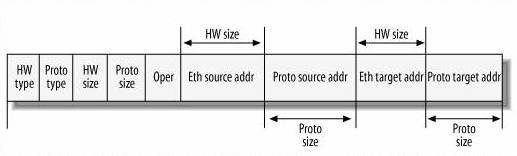
\includegraphics[width=300pt]{../imgs/arp.jpg}
\caption{Formato de una ARP.}
\end{center}
\end{figure}

Un ejemplo típico de uso podría ser el siguiente:\newline

\begin{quotation}
Una máquina en una red desea enviarle un paquete de datos a otra máquina de la misma red. Para eso, la máquina emisora busca, en su tabla local, la dirección MAC asociada a la dirección IP a la cuál desea mandar el paquete. Si no la encuentra, realiza el broadcast de la petición ARP, que llegará eventualmente si se encuentra conectada, a la máquina destino. 
La máquina destino recibirá la petición y responderá de manera unicast a la máquina que realizó la petición, poniendo en el paquete su dirección MAC para que la máquina destino de la respuesta pueda conocer la dirección MAC que necesitaba.
\end{quotation}

El análisis de la red consiste en reconocer su topología en base al nivel de información que proveen las diferentes IP, como fuente y como destino, tomando a las IP como símbolos y estimado su probabilidad de aparición con su frecuencia muestral. Para nuestro análisis, nos limitamos a la utilización de los paquetes $who-has$.

\section{Desarrollo}

Con el fin de obtener resultados relevantes, decidimos analizar redes Wi-Fi públicas de gran uso. Éstas fueron:

\begin{itemize}
\item CECEN-Wifi - Red pública del Pabellón II de Ciudad Universitaria, de gran utilización por parte de los estudiantes y docentes de la facultad.
\item Starbucks Núñez - Red pública utilizada por los clientes.
\item Red Empresarial - Con una magnitud aproximada de 30 dispositivos conectados en simultáneo.
\end{itemize}

Los tiempos de captura fueron los siguientes:

\begin{center}
  \begin{tabular}{| l | c |}
    \hline
    CECEN-Wifi & 23 minutos\\ \hline
    Starbucks & 50 minutos\\ \hline
    Red Empresarial & 30 minutos\\
    \hline
  \end{tabular}
\end{center}

Para la captura de paquetes, utilizamos Wireshark\footnote{http://www.wireshark.org} y Scapy\footnote{http://www.secdev.org/projects/scapy/}. Para la obtención de resultados, filtramos por redes ARP y $who-has$.

\section{Resultados}
Decidimos presentar los resultados obtenidos en forma de grafos dirigidos de IPs con pesos en los nodos (donde existe un eje entre la IP $x$ y la IP $y$ sí y sólo sí se observó un request ARP con source IP $x$ y target IP $y$). Para eso, modificamos su formato obtenido de la forma $IP_{src}\ \rightarrow \ IP_{dst} ;$ y utilizamos Graphviz\footnote{http://www.graphviz.org/}. Por otro lado, graficamos los histogramas de IPs solicitadas o grafos dirigidos de IPs con pesos en los nodos. De este modo, logramos analizar qué IPs son estadísticamente significativas en la LAN analizando la información de cada símbolo con respecto a la entropía de su respectiva fuente.

\subsection{CECEN-Wifi}

\subsection{Starbucks}

\subsection{Red Empresarial}


%\begin{figure}[H] %[h] Aqui [b] para button [t] para top
%\begin{center}
%\includegraphics[width=470pt]{../imgs/ej10_EDF03.png}
%\caption{Resultado de la simulación de EDF utilizando el lote descrito 
%anteriormente utilizando dos núcleos y los parámetros 2 0 0 SchedEDF.}


\section{Referencias}
\begin{itemize}
\item PETERSON, DAVIE ; Computer Networks, 5th edition, Wiley
\item STEVENS, W. Richard ; TCP/IP Illustrated, Volume 1

\item $http://wiki.wireshark.org/Gratuitous\_ARP$
\end{itemize}
\end{document}
